\documentclass[onecolumn,10pt]{jhwhw}

\usepackage{epsfig} %% for loading postscript figures
\usepackage{amsmath}
\usepackage{graphicx}
\usepackage{grffile}
\usepackage{pdfpages}
\usepackage{algpseudocode}
\usepackage{wrapfig}
\usepackage{pgfplots}
\usepackage{amsfonts}
\usepackage{booktabs}
\usepackage{siunitx}
\usepackage{commath}

% Default fixed font does not support bold face
\DeclareFixedFont{\ttb}{T1}{txtt}{bx}{n}{12} % for bold
\DeclareFixedFont{\ttm}{T1}{txtt}{m}{n}{12}  % for normal

% Custom colors
\usepackage{color}
\usepackage{listings}
\usepackage{framed}
\usepackage{caption}
\usepackage{bm}
\captionsetup[lstlisting]{font={small,tt}}

\definecolor{mygreen}{rgb}{0,0.6,0}
\definecolor{mygray}{rgb}{0.5,0.5,0.5}
\definecolor{mymauve}{rgb}{0.58,0,0.82}

\lstset{ %
  backgroundcolor=\color{white},   % choose the background color; you must add \usepackage{color} or \usepackage{xcolor}
  basicstyle=\ttfamily\footnotesize, % the size of the fonts that are used for the code
  breakatwhitespace=false,         % sets if automatic breaks should only happen at whitespace
  breaklines=true,                 % sets automatic line breaking
  captionpos=b,                    % sets the caption-position to bottom
  commentstyle=\color{mygreen},    % comment style
  deletekeywords={...},            % if you want to delete keywords from the given language
  escapeinside={\%*}{*)},          % if you want to add LaTeX within your code
  extendedchars=true,              % lets you use non-ASCII characters; for 8-bits encodings only, does not work with UTF-8
  frame=single,                    % adds a frame around the code
  keepspaces=true,                 % keeps spaces in text, useful for keeping indentation of code (possibly needs columns=flexible)
  columns=flexible,
  keywordstyle=\color{blue},       % keyword style
  language=R,                 % the language of the code
  % language=Python,                 % the language of the code
  morekeywords={*,...},            % if you want to add more keywords to the set
  numbers=left,                    % where to put the line-numbers; possible values are (none, left, right)
  numbersep=5pt,                   % how far the line-numbers are from the code
  numberstyle=\tiny\color{mygray}, % the style that is used for the line-numbers
  rulecolor=\color{black},         % if not set, the frame-color may be changed on line-breaks within not-black text (e.g. comments (green here))
  showspaces=false,                % show spaces everywhere adding particular underscores; it overrides 'showstringspaces'
  showstringspaces=false,          % underline spaces within strings only
  showtabs=false,                  % show tabs within strings adding particular underscores
  stepnumber=1,                    % the step between two line-numbers. If it's 1, each line will be numbered
  stringstyle=\color{mymauve},     % string literal style
  tabsize=4,                       % sets default tabsize to 2 spaces
}

\author{John Karasinski}
\title{Homework \# 7}

\begin{document}
%\maketitle

\problem{}
In your own words describe how RM ANOVA can be used to test for differences between groups, differences between repeated observations, and differences in observations as a function of group membership. These tests have specific names we discussed in lecture.\\

\begin{enumerate}
\item Groups Hypothesis (Test of Levels)
\begin{enumerate}
\item Do groups score similarly on the collected set of measures?
\item This test checks if the mean of the groups over all measurement times is the same. This does not mean that all the groups performed the same at each time point, just that their average performance is the same over all time points. Mathematically, this is simple measuring the relative contributions of between-group and within-group contributions to the total sum of squared errors. If the group `levels' are significantly different, then the equal levels null hypothesis is rejected.
\end{enumerate}
\item Flatness Hypothesis (Test of Flatness)
\begin{enumerate}
\item Is the dependent variable similar across assessments?
\item This test checks if the difference in the response between assessments (i.e., the slope) is nonzero. The flatness null hypothesis is that the slope between all assessments is zero, and that the results are flat. This is checked for each group, and is effectively a within-subjects test. If the slope is statistically significantly nonzero, then there is a within groups main effect of time.
\end{enumerate}
\item Parallelism Hypothesis (Test of Parallelism)
\begin{enumerate}
\item Do different groups have parallel profiles?
\item This test checks if the slope between each set of assessments is the same across all groups. This is equivalent to a one-way ANOVA on the slopes, we are checking that there is no interaction of the within-subjects factor with the between-subjects factor.
\end{enumerate}
\end{enumerate}

\problem{}
Why do we say that in RM ANOVA time is treated as a categorical variable?

RM ANOVA treats time as a categorical factor. Time is considered a set of discrete, fixed conditions in which each subject contributes one outcome variable per time condition. The ANOVA model for describing mean change over time uses as many parameters as there are discrete occasions. This is also known as a saturated means model---the model for time is saturated by using all possible degrees of freedom for differences across conditions of the time variable. The goal of the ANOVA model is not to predict or summarize the pattern of means, but simply to reproduce the observed mean per occasion using fixed effects equal to the number of occasions minus 1 (given that the fixed intercept is already included).

\problem{}
What is the difference between polynomial contrasts and comparisons of means between different observation periods?

Polynomial contrast can be used to test which level of polynomial (linear, quadratic, cubic) explains the relation under study. The comparison of means between different observation periods doesn't lead to information about how the dependent variable changes with time, just that there may be some difference between the observations (e.g. categorical differences). In that respect, polynomial contrasts can give the statistician more information about the underlying variable.

\problem{}
Researchers were interested in how confidence in students fluctuates from the end of sophomore year through the end of senior year in college. Further, researchers were interested in whether students attended a private (i.e., Harvard, Stanford, and Yale) or public (i.e., UMass---Boston, San Francisco State University, and Southern Connecticut State University) university would influence end-of-year student confidence ratings, and possible trajectories.

Use the data set “confidence.csv” to answer the following questions. For your information, t1-t3 indicate time of observation 1-3; i.e., end of sophomore year, end of junior year, and end of senior year, respectively. The variable public indicates whether the student attended a public (public = 1) or private (public = 0) university.\\

\noindent1. Convert the wide format data set to a long format data set. Remember that you will need to create an ID variable, and an Observation/Time variable. Show syntax and the header and footer of the long format data set.\\

% \begin{lstlisting}
% import pandas as pd

% df = pd.read_csv('confidence.csv')

% # Convert to long format
% r = pd.melt(df.reset_index(),
%             value_vars=['t1', 't2', 't3'],
%             id_vars=['index', 'public'],
%             var_name='Time', value_name='Observation')

% # Some basic sorting
% r = r.sort(['index', 'Time']).reset_index(drop=True)

% # Rename first column to ID
% cols = r.columns.tolist()
% cols[0] = 'ID'
% r.columns = cols

% # Print head and tail of new dataframe
% print(r.head())
% print(r.tail())
% \end{lstlisting}

\begin{lstlisting}
# Load data
gwide <- read.csv("confidence.csv")

# Convert from wide to long format
public <- rep(c(0, 1), each = 150)
obs <- rep(c("t1", "t2", "t3"), 100)
time <- rep(c(0.5, 1.5, 2.5), 100)
id <- paste("id", 1:100, sep = "")
observation <- unlist(lapply(1:100, function(x) {gwide[x, 1:3]}))
glong <- data.frame(id, obs, time, public, observation)
> head(glong)
   id obs time public observation
1 id1  t1  0.5      0           4
2 id2  t2  1.5      0           6
3 id3  t3  2.5      0           6
4 id4  t1  0.5      0           3
5 id5  t2  1.5      0           5
6 id6  t3  2.5      0           5
> tail(glong)
       id obs time public observation
295  id95  t1  0.5      1           3
296  id96  t2  1.5      1           4
297  id97  t3  2.5      1           4
298  id98  t1  0.5      1           4
299  id99  t2  1.5      1           5
300 id100  t3  2.5      1           4
\end{lstlisting}
% \noindent OUTPUT
% \begin{lstlisting}[language={}]
%    ID  public Time  Observation
% 0   0       0   t1            4
% 1   0       0   t2            6
% 2   0       0   t3            6
% 3   1       0   t1            3
% 4   1       0   t2            5

%      ID  public Time  Observation
% 295  98       1   t2            4
% 296  98       1   t3            4
% 297  99       1   t1            4
% 298  99       1   t2            5
% 299  99       1   t3            4
% \end{lstlisting}

\noindent2. Test whether public and private universities differed in their confidence scores. Conduct any pairwise comparison necessary. Report your conclusions.\\

% \begin{lstlisting}
% print(anova_lm(ols("Observation ~ C(public)", df.groupby('ID').mean()).fit()))
% \end{lstlisting}
\begin{lstlisting}
> summary(aov(observation ~ public + Error(id), data = glong))

Error: id
          Df Sum Sq Mean Sq F value Pr(>F)
public     1   2.43   2.430   1.689  0.197
Residuals 98 140.97   1.438

Error: Within
           Df Sum Sq Mean Sq F value   Pr(>F)
public      1  47.04   47.04    30.5 1.04e-07 ***
Residuals 199 306.96    1.54
---
\end{lstlisting}
% \noindent OUTPUT
% \begin{lstlisting}[language={}]
%            df      sum_sq    mean_sq          F    PR(>F)
% C(public)   1   16.267778  16.267778  15.910954  0.000128
% Residual   98  100.197778   1.022426        NaN       NaN
% \end{lstlisting}

A one-way between subjects ANOVA was conducted to compare the effect of different types of universities on student confidence for students at public and private universities. There was not a significant effect of university type on student confidence at the $p=0.05$ level for the two conditions $[F(1, 98)=1.7, p =0.197]$. Comparisons of the mean indicated that the mean confidence scores for the private university students $(M=3.77, SD=1.30)$ was larger than the public university students $(M=2.96, SD=1.15)$.\\

\noindent3. Test whether confidence differs over time. Do this by comparing all observations to each other. Also do this by testing the maximum allowable number of polynomial contrasts. Report your conclusions for both tests.\\

% \begin{lstlisting}
% from patsy import dmatrix

% # This is equivalent to R's contr.poly
% p = dmatrix("C(df.Time, Poly())", df)
% poly = pd.DataFrame(p, columns=['Intercept', 'Linear', 'Quadratic'])
% df = pd.concat((df, poly), axis=1)
% print(anova_lm(ols("Observation ~ C(Time)", data=df).fit()))
% print(MultiComparison(df.Observation, df.Time).allpairtest(ttest_ind, method='b')[0])
% print(anova_lm(ols("Observation ~ Linear + Quadratic", data=df).fit(), typ=2))
% \end{lstlisting}
% \noindent OUTPUT
% \begin{lstlisting}[language={}]
%            df      sum_sq   mean_sq         F    PR(>F)
% C(Time)     2   13.406667  6.703333  4.113494  0.017291
% Residual  297  483.990000  1.629596       NaN       NaN

% Test Multiple Comparison ttest_ind
% FWER=0.05 method=b
% alphacSidak=0.02, alphacBonf=0.017
% =============================================
% group1 group2   stat   pval  pval_corr reject
% ---------------------------------------------
%   1      2    -3.3552 0.001    0.0029   True
%   1      3    -2.0881 0.0381   0.1142  False
%   2      3     0.4905 0.6243    1.0    False
% ---------------------------------------------

%                sum_sq   df         F    PR(>F)
% Linear       7.605000    1  4.666801  0.031551
% Quadratic    5.801667    1  3.560187  0.060156
% Residual   483.990000  297       NaN       NaN
% \end{lstlisting}

\begin{lstlisting}
> # Test for effect of observation
> summary(aov(observation ~ obs + Error(id), data = glong))

Error: id
          Df Sum Sq Mean Sq F value Pr(>F)
Residuals 99  143.4   1.448

Error: Within
           Df Sum Sq Mean Sq F value Pr(>F)
obs         2   13.4   6.703   3.897 0.0219 *
Residuals 198  340.6   1.720
---
>
> pairwise.t.test(glong$observation, glong$obs,paired = TRUE, p.adjust = c("bonf"))

  Pairwise comparisons using paired t tests
data:  glong$observation and glong$obs
   t1      t2
t2 1.7e-06 -
t3 0.024   1.000
P value adjustment method: bonferroni
\end{lstlisting}

A one-way within subjects ANOVA was conducted to compare the effect of time on student confidence. There was a significant effect of time on student confidence at the $p=.05$ level for the three conditions $[F(2, 198) = 3.9, p = 0.02]$. Post-hoc t-tests at the $p=.05$ level with the Bonferroni correction indicated that there was a significant difference between measurements at time 1 and 2, and time 1 and 3, but not between time 2 and 3.\\

\begin{lstlisting}
> # Add Polynomial Contrasts to describe trajectories
> glong[, 6] <- contr.poly(3)[, 1]
> glong[, 7] <- contr.poly(3)[, 2]
>
> colnames(glong) <- c(colnames(glong[, 1:5]), c("l", "q"))
>
> # Test to see linear/quadratic contrasts describe the observations
> summary(aov(observation ~ l + q + Error(id), data = glong))

Error: id
          Df Sum Sq Mean Sq F value Pr(>F)
Residuals 99  143.4   1.448

Error: Within
           Df Sum Sq Mean Sq F value Pr(>F)
l           1    7.6   7.605   4.421 0.0368 *
q           1    5.8   5.802   3.373 0.0678 .
Residuals 198  340.6   1.720
---
\end{lstlisting}

Polynomial contrasts were also investigated to explain the relation between time and student confidence scores at the $p=0.05$ level. There was a significant linear trend, $[F(1, 198) = 4.4, p = 0.04]$, indicating that as time increased, the student confidence scores increased proportionally. A quadratic trend was also investigated, but was found to be non-significant, $[F(1, 198) = 3.4, p = 0.07]$.\\

\noindent4. Test for a possible interaction between variables tested in question 2 (university type) and 3 (mean differences between observations and significant trends in confidence). Conduct any follow-up analyses necessary if there is a significant interactions. Report your conclusions for all tests.

\begin{lstlisting}
> # Test for interaction effect
> summary(aov(observation ~ public:obs + Error(id), data = glong))
Error: id
           Df Sum Sq Mean Sq F value   Pr(>F)
public:obs  3  32.87  10.958   9.518 1.45e-05 ***
Residuals  96 110.52   1.151
---

Error: Within
            Df Sum Sq Mean Sq F value   Pr(>F)
public:obs   3  52.39  17.464   11.41 6.26e-07 ***
Residuals  197 301.61   1.531

# Output truncated for follow-up tests

# Follow-up options Simple Effects split on interaction: e.g., public vs. private
summary(aov(observation ~ obs + Error(id), glong[which(glong$public == 0), ]))
summary(aov(observation ~ obs + Error(id), glong[which(glong$public == 1), ]))

# Test where differences exist
pairwise.t.test(glong[which(glong$public == 1), "observation"],
                glong[which(glong$public == 1), "obs"],
                paired = TRUE, p.adjust = c("bonf"))
pairwise.t.test(glong[which(glong$public == 0), "observation"],
                glong[which(glong$public == 0), "obs"],
                paired = TRUE, p.adjust = c("bonf"))

# Follow-up options Simple Effects split on Observation
summary(aov(observation ~ public + Error(id), glong[which(glong$obs == 't1'), ]))
summary(aov(observation ~ public + Error(id), glong[which(glong$obs == 't2'), ]))
summary(aov(observation ~ public + Error(id), glong[which(glong$obs == 't3'), ]))

# Find mean and sd
t3 = glong[glong$time == 2.5,]
aggregate(t3$observation, by=list(t3$public), FUN=mean)
aggregate(t3$observation, by=list(t3$public), FUN=sd)
\end{lstlisting}

A one-way between subjects ANOVA was conducted to test for an interaction between university type and observation on student confidence. There was a significant interaction detected at the $p=0.05$ level $[F(3, 96)=9.5, p <.001]$. Follow-up simple effects analyses indicated that there was a significant effect of observation for both private $[F(2, 97)=29.7, p <.001]$ and public $[F(2, 97)=5.2, p =.001]$ schools. Pairwise t-tests for both private and public schools indicated significant differences among all combinations of observation periods. Simple effects analyses also show a simple effect for the third observation $[F(1, 98)=44.1, p <.001]$. Student confidence scores in the third observation were significantly higher for the students in private schools $(M=4.38, SD=1.50)$ than public school $(M=2.54, SD=1.27)$.

% \begin{lstlisting}
% print(anova_lm(ols("Observation ~ C(Time)*C(public)", data=df).fit(), typ=2))

% # Test for simple effects
% print(anova_lm(ols("Observation ~ C(Time)", data=df.query('public == 0')).fit(), typ=2))
% print(anova_lm(ols("Observation ~ C(Time)", data=df.query('public == 1')).fit(), typ=2))
% print(anova_lm(ols("Observation ~ C(public)", data=df.query('Time == 1')).fit(), typ=2))
% print(anova_lm(ols("Observation ~ C(public)", data=df.query('Time == 2')).fit(), typ=2))
% print(anova_lm(ols("Observation ~ C(public)", data=df.query('Time == 3')).fit(), typ=2))
% \end{lstlisting}
% \noindent OUTPUT
% \begin{lstlisting}[language={}]
%                        sum_sq   df          F        PR(>F)
% C(Time)             13.406667    2   4.995134  7.356729e-03
% C(public)           48.803333    1  36.366858  4.897455e-09
% C(Time):C(public)   40.646667    2  15.144371  5.496327e-07
% Residual           394.540000  294        NaN           NaN

%               sum_sq   df          F    PR(>F)
% C(Time)    37.213333    2  12.685187  0.000008
% Residual  215.620000  147        NaN       NaN

%           sum_sq   df        F    PR(>F)
% C(Time)    16.84    2  6.91784  0.001345
% Residual  178.92  147      NaN       NaN

%            sum_sq  df         F    PR(>F)
% C(public)    0.81   1  1.107113  0.295298
% Residual    71.70  98       NaN       NaN

%            sum_sq  df         F    PR(>F)
% C(public)    4.00   1  2.911468  0.091119
% Residual   134.64  98       NaN       NaN

%            sum_sq  df          F        PR(>F)
% C(public)   84.64   1  44.073964  1.766331e-09
% Residual   188.20  98        NaN           NaN
% \end{lstlisting}

\begin{table}[h!]
\begin{center}
\begin{tabular}{l r r r r r}
\toprule
Source & $SS$ & $df$ & $F$ & $PR(>F)$ \\
\midrule
\it{School Type} & & & & \\
\hspace{1em} Private     & 29.66 &  2  & 11.97 & $<.001$ \\
\hspace{1em} Public      & 13.69 &  2  &  5.18 & $ .001$ \\
\it{Time} & & & & \\
\hspace{1em} 1      &  0.81 &  1  &  1.1 & $ .295$\\
\hspace{1em} 2      &  4.00 &  1  &  2.9 & $ .091$\\
\hspace{1em} 3      & 84.64 &  1  & 44.1 & $<.001$\\
\bottomrule
\end{tabular}
\end{center}
\caption{Results of Simple Effects Analysis}
\end{table}

\clearpage
\noindent5. Create a plot of the data that represents the trajectory for public and private students. Make sure the trajectories have some indication of variability around the average trajectory. Sufficiently label and describe your figure.\\

\begin{lstlisting}[language=Python]
# Python!
import pandas as pd
import seaborn as sns
sns.set_style('ticks')

df = pd.read_csv('glong.csv', index_col=0)
p = sns.lmplot(x='time', y='observation',
               hue='public',
               data=df, order=2, ci=95,
               x_jitter=.3, y_jitter=.3,
               markers=["o", "x"],
               legend=False)
p.axes[0][0].set_xticks([0.5, 1.5, 2.5])
p.axes[0][0].set_xticklabels(['Sophomore', 'Junior', 'Senior'])
plt.xlabel('Observation')
plt.ylabel('End-of-Year Student Confidence Rating')
plt.savefig('prob5-quad.pdf')
plt.close('all')
\end{lstlisting}

% \begin{figure}[h!]
% \begin{center}
% 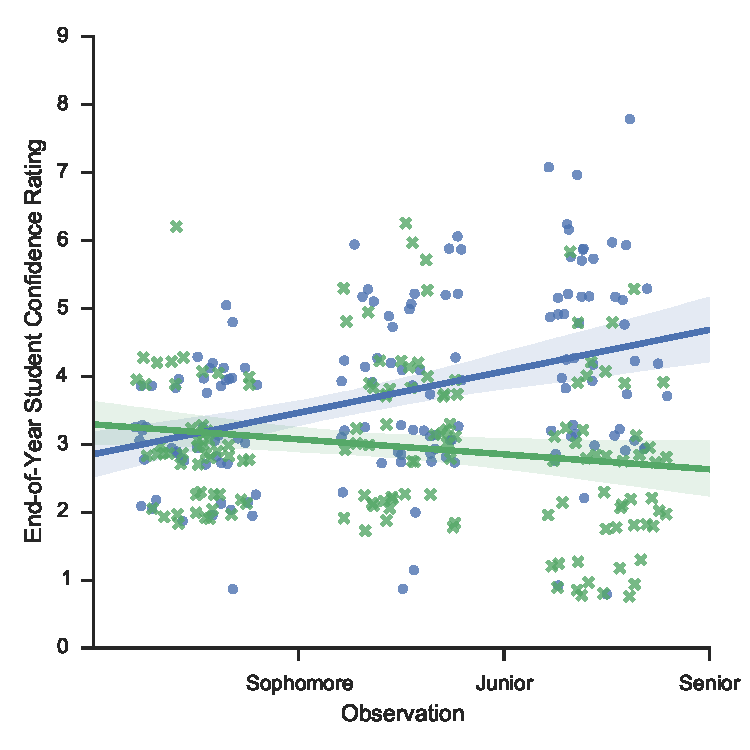
\includegraphics[width=.5\textheight]{prob5-lin.pdf}
% \label{fig:on}
% \end{center}
% \caption{Linear trajectories for end-of-year confidence ratings for students in public schools (green) and private schools (blue). Shaded regions represent 95\% confidence regions. (Some jitter introduced for visibility.)}
% \end{figure}

This figure shows a scatter plot of each observation of student confidence ratings. The ratings of public school students are shown as green x's, and blue o's represent the private schools. As the dataset contains only three distinct measurement conditions and eight observation values, a small amount of jitter is added to each observation. This jitter allows the viewer to get a better idea of how many data points are at each location. The quadratic fit to the public and private schools is overlaid on the scatter plot along with 95\% confidence regions. Private schools show an overwhelmingly linear fit, while public schools shown a quadratic fit which slopes downward in the final observation category, making the interaction evident.

\begin{figure}[h!]
\begin{center}
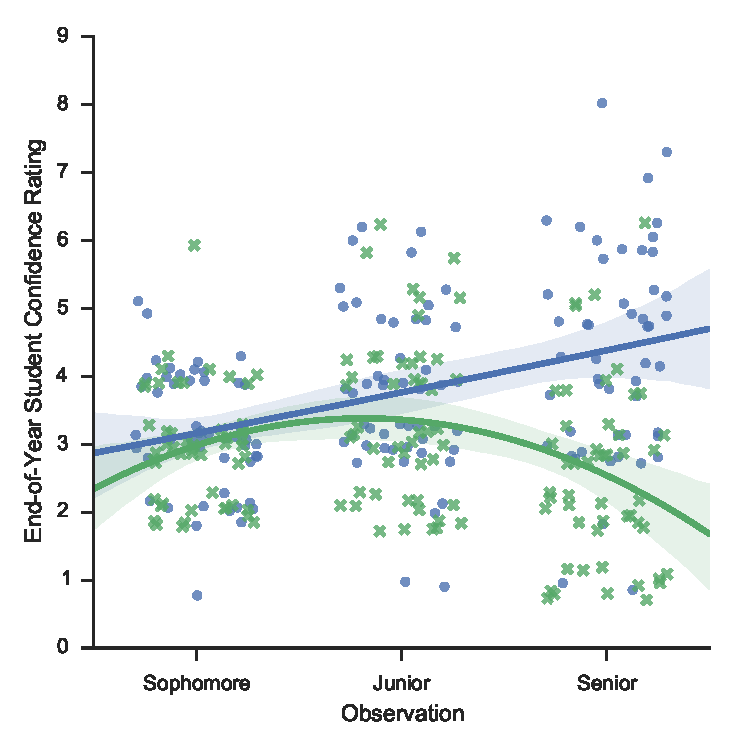
\includegraphics[width=1\textwidth]{prob5-quad.pdf}
\label{fig:on}
\end{center}
\caption{Quadratic trajectories for end-of-year confidence ratings for students in public schools (green) and private schools (blue). Shaded regions represent 95\% confidence regions. (Some jitter introduced for visibility.)}
\end{figure}


\end{document}
